
\chapter{Methodology}

\acresetall

The algorithms outlined throughout the following chapter were implemented
in MATLAB. This environment was selected due to its availability and
ease-of-use. MATLAB includes a number of tools useful in signal processing
and statistical analysis \citep{Krauss1994,Jones1997}, and other
authors have provided tools in the MATLAB language \citep{Hoyer2004,Brookes1997,Loizou2008,Wojcicki2011}.
A limitation of the MATLAB environment in signal processing is the
comparative performance with lower-level languages, however performance
and speed were not a primary focus in this thesis, so this was deemed
acceptable.

Data analysis was conducted using the R programming language \citep{RCoreTeam2014}.
R was selected for data analysis for its simplicity in forming powerful
plots and applying statistical methods.

Simulations were run on a MacBook Pro 64-bit system with an Intel
Core i7 2.3GHz 4-core processor with 16GB memory, running OSX 10.9.2,
MATLAB R2013a and R version 3.1.0 (2014-04-10).

Test data was drawn from the \ac{WSJ} corpus \citep{Robinson1995}.
Different recordings were reserved for testing and training. Babble
noise was simulated by using recordings of speech, also drawn from
the \ac{WSJ} corpus. Additionally, recorded noise was used from the
NOIZEUS corpus \citep{Hu2006}.


\section{Humanly Perceived Improvement vs. Machine Performance}

The first research area sought to answer the research question \ref{enu:ResQ1},
\textit{\RQone{}} The focus was to compare and contrast the performance
differences of speech enhancement algorithms when evaluated on a human
listener versus a machine listener.


\subsection{\label{sub:Method-Existing-Data}Investigating Existing Data}

Data on enhancement performance of various algorithms and under different
measures of enhancement was collected from a number of sources \citep{mohammadiha2013supervised,Wilson2008,Schmidt2006,Raj2005,Rennie2008,Weninger2011,Williamson2014,Paliwal2010,Plourde2007}
and is presented in \chapref{Apx-Data}, \secref{litresults}. As
noted in \chapref{Literature-Review} \textit{\nameref{chap:Literature-Review}},
most literature takes preference to evaluation measures indicative
of either human performance or machine performance, but not both.
Thus, a method had to be developed in order to fairly compare the
the results between different sources.

This method involved plotting human performance against machine performance,
and thus was only applicable to a small subset of available results
where both performances were measured, such as in \citep{Paliwal2010}.
This data was analysed separately for each type of algorithm investigated.
Each data set had a \ac{LOESS} model fitted, in order to quickly
and visually judge the accuracy of applying a \ac{LM} fit. An \ac{LM}
model fit was then applied using R's \lstinline[language=R]!lm()!
linear regression function. The main limitation of the direct comparison
method was the limited dataset available.


\subsection{\label{sub:Independent-Investigation-Meth}Independent Investigation}

Due to the lack of existing data on which conclusions can be drawn
on the human vs. machine success of various speech enhancement algorithms,
independent tests were required to be run. In order to answer the
research question, a number of enhancement algorithms were required
to be used to enhance speech, and a number of evaluation measures,
of both human perceptual and machine recognition types, were to be
used to measure the performance.

The Algorithms used in testing are given in \tabref{Algorithms},
and the noise types used are given in \ref{tab:test-params}. The
first seven tests consisted of synthetic babble, test nine was a recorded
babble, and tests seven and ten were recordings of mixed noise types
which included speech type noise along with other noise types. The
last three noise types were drawn from the NOIZEUS corpus presented
in \citep{Hu2006}.

\begin{table}


\protect\caption{\label{tab:Algorithms}Algorithms used in testing}


\begin{tabular*}{1\textwidth}{@{\extracolsep{\fill}}|>{\raggedright}p{0.15\textwidth}|>{\raggedright}p{0.6\textwidth}|>{\raggedright}p{0.13\textwidth}|}
\hline 
Name & Description & Code\tabularnewline
\hline 
\hline 
Mohammadia Supervised & A supervised \ac{BNMF} algorithm proposed in \citep{mohammadiha2013supervised},
trained on simple utterances of the \ac{SoI}. & \lstref{mohammadiaSupervised}\tabularnewline
\hline 
Phoneme Mohammadia Supervised & A supervised \ac{BNMF} algorithm proposed in \citep{mohammadiha2013supervised},
trained on drawn phoneme samples of the \ac{SoI}. See \subsecref{Phoneme-Training}. & \lstref{mohammadiaSupervised}\tabularnewline
\hline 
Mohammadia Online & An online \ac{BNMF} algorithm proposed in \citep{mohammadiha2013supervised},
trained on simple utterances of the \ac{SoI}. & \lstref{mohammadiaOnline}\tabularnewline
\hline 
Phoneme Mohammadia Online & An online \ac{BNMF} algorithm proposed in \citep{mohammadiha2013supervised},
trained on drawn phoneme samples of the \ac{SoI}. See \subsecref{Phoneme-Training}. & \lstref{mohammadiaOnline}\tabularnewline
\hline 
Modified Supervised & A modified supervised \ac{BNMF} method using explicitly phoneme \ac{NMF}
bases. See \subsecref{Phoneme-Base}. & \lstref{modifiedSupervised}\tabularnewline
\hline 
Modified Online & A modified online \ac{BNMF} method using explicitly phoneme \ac{NMF}
bases. See \subsecref{Phoneme-Base}. & \lstref{modifiedOnline}\tabularnewline
\hline 
\acs{MMSE} & A spectral subtraction algorithm with \ac{MMSE} error estimation,
\lstinline[language=Matlab]!ssubmmse()! in \citep{Brookes1997},
trained on simple utterances of the \ac{SoI}. & \lstref{MMSE}\tabularnewline
\hline 
Phoneme \acs{MMSE} & A spectral subtraction algorithm with \ac{MMSE} error estimation,
\lstinline[language=Matlab]!ssubmmse()! in \citep{Brookes1997},
trained on simple drawn phoneme samples of the \ac{SoI}. & \lstref{MMSE}\tabularnewline
\hline 
Ideal Binary Mask & A ideal binary mask algorithm \citep{Wojcicki2011}, trained on simple
utterances of the \ac{SoI}. & \lstref{IDBM}\tabularnewline
\hline 
Phoneme Ideal Binary Mask & A ideal binary mask algorithm \citep{Wojcicki2011}, trained on simple
drawn phoneme samples of the \ac{SoI}. & \lstref{IDBM}\tabularnewline
\hline 
\end{tabular*}
\end{table}


\begin{table}
\protect\caption{\label{tab:test-params}Simulations and associated parameters}


\centering{}%
\begin{tabular}{|c|c|c|}
\hline 
Test Number & \ac{SoI} (sex) & Noise\tabularnewline
\hline 
\hline 
1 & C3C (f) & Competing speaker: C3F (m)\tabularnewline
\hline 
2 & C3L (f) & Competing speaker: C31 (m)\tabularnewline
\hline 
3 & C3S (m) & Competing speaker: C31 (m)\tabularnewline
\hline 
4 & C3S (m) & Synthetic babble: C31 (m) + C34 (m) + C35 (m)\tabularnewline
\hline 
5 & C3S (m) & Synthetic babble: C3F (m) + C3C (f) + C35(m)\tabularnewline
\hline 
6 & C3S (m) & Synthetic babble: C3F (m) + C3C (f)\tabularnewline
\hline 
7 & C3S (m) & Competing speaker: C3F(m)\tabularnewline
\hline 
8 & C3S (m) & NOIZEUS car\tabularnewline
\hline 
9 & C3S (m) & NOIZEUS babble\tabularnewline
\hline 
10 & C3S (m) & NOIZEUS street\tabularnewline
\hline 
\end{tabular}
\end{table}


The performance measures used were \ac{PESQ} \citep{InternationalTelecommunicationUnion2001},
\ac{MOS}, \ac{CCR} \citep{InternationalTelecommunicationUnion1996},
\ac{PRR} and segmental \ac{SNR}.


\subsubsection*{Objective Measures of Quality}

\ac{PESQ} was selected as a performance measure due to its extensive
usage in literature. Using the same evaluation measure allowed a certain
degree of comparability with others' results. The \ac{PESQ} implementation
used was a MATLAB implementation provided by \citet{Loizou2008}.

Segmental \ac{SNR} was also selected as a performance measure in
order to incorporate a statistical measure. A MATLAB implementation
was also supplied with \citep{Loizou2008}, so implementation was
straightforward.


\subsubsection*{Testing on Human Subjects}

\ac{MOS} and \ac{CCR} were selected due to their subjective qualities.
Although subjective measures are generally avoided, they were decided
to be useful in the experimental context, as human perception is itself
subjective. \ac{MOS}, like \ac{PESQ}, had been used throughout literature,
and so was included as a test measure for comparability. \ac{CCR}
was included also since the scale used lent itself to measuring enhancement,
and is in many ways more similar to \ac{PESQ} due to the fact it
measures improvement or degradation from a reference.

A MATLAB implementation of the \ac{MOS} test exists \citep{Ruzanski2009},
however the implementation was not flexible and the script was not
found to be suited to the required test. A new \ac{MOS} and \ac{CCR}
script was created, in alignment with the requirements outlined by
the \citet{InternationalTelecommunicationUnion1996}. The resulting
code is given in \cref{lst:MOSScript,lst:MOS}, and has been submitted
to MATLAB Central and GitHub to share with the community \citep{Gillman2014}.

The scales used are given in \tabref{MOS-CCR-Scales}. Two \ac{MOS}
scales were used, one measuring quality opinion, and one measuring
required effort opinion.

\begin{table}[h]
\protect\caption{\label{tab:MOS-CCR-Scales}Scales used in subjective tests}


\begin{centering}
\subfloat[\acs{MOS} listening quality scale]{

\centering{}%
\begin{minipage}[t]{1\columnwidth}%
\begin{center}
\begin{tabular}{|c|c|}
\hline 
Quality of the speech & Score\tabularnewline
\hline 
\hline 
Excellent & 5\tabularnewline
\hline 
Good & 4\tabularnewline
\hline 
Fair & 3\tabularnewline
\hline 
Poor & 2\tabularnewline
\hline 
Bad & 1\tabularnewline
\hline 
\end{tabular}
\par\end{center}%
\end{minipage}}
\par\end{centering}

\begin{centering}
\subfloat[\acs{MOS} listening effort scale]{

\centering{}%
\begin{minipage}[t]{1\columnwidth}%
\begin{center}
\begin{tabular}{|c|c|}
\hline 
Effort required to understand the meanings of sentences & Score\tabularnewline
\hline 
\hline 
Complete relaxation possible; no effort required & 5\tabularnewline
\hline 
Attention necessary; no appreciable effort required & 4\tabularnewline
\hline 
Moderate effort required & 3\tabularnewline
\hline 
Considerable effort required & 2\tabularnewline
\hline 
No meaning understood with any feasible effort & 1\tabularnewline
\hline 
\end{tabular}
\par\end{center}%
\end{minipage}}
\par\end{centering}

\centering{}\subfloat[\acs{CCR} scale]{\begin{centering}

\par\end{centering}

\centering{}%
\begin{minipage}[t]{1\columnwidth}%
\begin{center}
\begin{tabular}{|c|c|}
\hline 
The quality of the second compared to the quality of the first & Score\tabularnewline
\hline 
\hline 
Much Better & 3\tabularnewline
\hline 
Better & 2\tabularnewline
\hline 
Slightly Better & 1\tabularnewline
\hline 
About the Same & 0\tabularnewline
\hline 
Slightly Worse & -1\tabularnewline
\hline 
Worse & -2\tabularnewline
\hline 
Much Worse & -3\tabularnewline
\hline 
\end{tabular}
\par\end{center}%
\end{minipage}}
\end{table}


When performing the \ac{MOS} and \ac{CCR} tests, some of the recommendations
could not be met. Sound-proof rooms were not available, as recommended
in \citep{InternationalTelecommunicationUnion1996} Annex A, and so
environmental, room and vehicle noise were not able to be tightly
controlled. However, an internal room, i.e., with no exterior walls,
was available. Measurements taken on a Samson Meteor condenser microphone
showed the environmental noise to be at an acceptable level, as seen
in \figref{Typical-noise-level}.

\begin{figure}
\begin{centering}
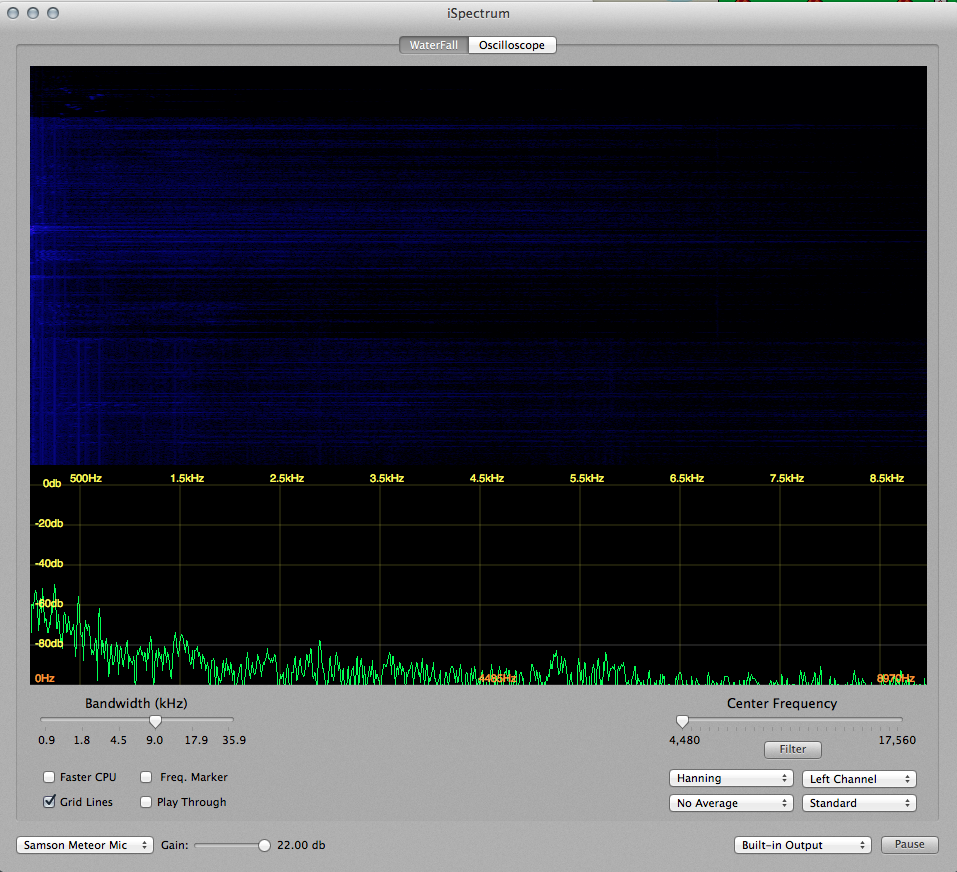
\includegraphics[width=0.8\textwidth]{fig/environment}
\par\end{centering}

\protect\caption{\label{fig:Typical-noise-level}Typical noise level during tests}
\end{figure}




The test setup is depicted in \figref{MOS-Test-setup}. The setup
was located in the aforementioned interior room. The test was performed
on a laptop running the MATLAB code (\lstref{MOSScript}), and the
test subject listened using a pair of over-ear headphones. Studio
quality headphones were not available, so Pioneer SE-MJ711 headphones
were used. The test procedure went as follows:
\begin{enumerate}
\item The subject was shown a recording of the \ac{SoI} so that they could
identify which speaker was the intended speaker in competing speaker
noise situations.
\item The test procedure was described to the subject, noting that three
separate tests were to be performed, meaning the subject would be
asked three types of questions.
\item With the laptop playing audio through the speakers, the test was begun
and the test coordinator showed the subject how to use the program,
running through approximately two iterations of the test.
\item The subject was then given headphones and instructed to start the
test.
\item The test coordinator was required to remain with the subject for the
duration of the test to answer any questions.
\end{enumerate}
\begin{figure}
\begin{centering}
\includegraphics[width=0.8\textwidth]{\string"fig/test setup\string".jpg}
\par\end{centering}

\protect\caption{\label{fig:MOS-Test-setup}MOS Test setup}
\end{figure}


\tabref{MOS-Subject-summary} gives a summary of the ten test subjects
that were used in gathering the \ac{MOS} results. Test subjects were
selected to give a range in age and sex. Also included in the test
subjects was a listener with a hearing disability, pulsative tinitis,
who was a hearing aid user.

\begin{table}
\protect\caption{\label{tab:MOS-Subject-summary}Summary of test subjects use in \ac{MOS}
test}


\centering\csvautotabular{dat/TestSubjects.csv}
\end{table}



\subsubsection*{\acl{ASR}}

Both \ac{HTK} and Sphinx were both considered for the \ac{ASR} system
for the \ac{PRR} results. Both offer comparable performance in recognition
and processing performance \citep{Vertanen2006}. \ac{HTK} was used
due to an availability of experience within the university. The chosen
\ac{ASR} method was a \ac{MFCC} feature vector. The selected training
data was the full recording set for the \ac{SoI}.

The script to implement the \ac{HTK} setup, training, extraction
and evaluation steps was based on that developed by \citet{Quill2014},
and is given in \ref{lst:ASR}. A basic overview of the script's function
is given in \algref{ASR}. The parameters used in performing the \ac{MFCC}
domain \ac{ASR} are given in \cref{lst:MFC-config,lst:MFC-proto}.

\begin{algorithm}
\begin{enumerate}
\item Setup

\begin{enumerate}
\item Collate all test data into one folder, with a standard naming convention.
\item Produce required metadata on training data, including phoneme lists,
grammar rules, file lists, transcription summaries, etc.
\item Initialise empty initial \acp{HMM} using \ac{HTK}'s \lstinline[language=bash]!HVITE!,
based on a user defined configuration and prototype for the desired
feature vectors. In this case, these were those given in \cref{lst:MFC-config,lst:MFC-proto}.
\end{enumerate}
\item Training

\begin{enumerate}
\item Convert training data to \ac{MFCC} domain using \ac{HTK}'s \lstinline[language=bash]!HCOPY!.
\item The \ac{HMM} model is then re-estimated twice, using \ac{HTK}'s
\lstinline[language=bash]!HEREST!.
\item The \ac{HMM} model is then re-estimated a further three times, this
time incorporating a short pause model but still using \lstinline[language=bash]!HEREST!.
\item The phoneme transcriptions are realigned using the current model and
\ac{HTK}'s \lstinline[language=bash]!HVITE!. The \ac{HMM} model
is then re-estimated yet another three times still using \lstinline[language=bash]!HEREST!.
\end{enumerate}
\item Extraction

\begin{enumerate}
\item Convert test data to \ac{MFCC} domain using \ac{HTK}'s \lstinline[language=bash]!HCOPY!.
\item Perform recognition and generate an estimated phoneme transcription
using \ac{HTK}'s \lstinline[language=bash]!HVITE!.
\end{enumerate}
\item Evaluation

\begin{enumerate}
\item Use \ac{HTK}'s \lstinline[language=bash]!HRESULTS! to compare the
estimated phoneme transcription with the original phoneme transcription.
\end{enumerate}
\end{enumerate}
\protect\caption{\label{alg:ASR} \acs{ASR} with \acs{HTK}}
\end{algorithm}


\begin{listing}[H]
\protect\caption{\acs{MFCC} configuration file\label{lst:MFC-config}}


\lstinputlisting[nolol=true,style=myBash]{../Code/python/MFC_HCompV_Config.ini}
\end{listing}


\begin{listing}[H]
\protect\caption{\acs{MFCC} prototype file\label{lst:MFC-proto}}


\lstinputlisting[nolol=true,style=myBash]{../Code/python/MFCProto}
\end{listing}



\section{Assessing \acl{NMF} Algorithm Training}

The second research area sought to answer research question \ref{enu:ResQ2},
\textit{\RQtwo{}} The focus was to investigate the training requirements
of supervised speech enhancement algorithms, and to investigate means
of improving the quality of training.


\subsection{\label{sub:Investigating-Training-Req}Investigating Training Requirements}

An experiment was conducted, investigating the effects of the performance
of enhancement. Firstly, test data was generated, using the code given
in \lstref{createTestData}, \textit{\nameref{lst:createTestData}}.
The data was formed as \lstinline[language=bash]!.wav! files consisting
of:
\begin{itemize}
\item training files, for use by supervised enhancement algorithms, for
both \ac{SoI} and noise recordings;
\item test files, or dirty files, for the enhancement algorithms to operate
on;
\item the clean file, for the evaluation algorithms to compare the enhancement
with; and
\item the clean noise file.
\end{itemize}
A range of training files were created, varying the number of utterances
included. The \ac{WSJ} corpus included 90 utterances per speaker%
\footnote{There are 90 utterances for the speakers reserved for training, \lstinline[language=bash]!si_dt!,
which were used in this test.%
} \citep{Fransen1994}, so 10 utterances were used for the test speech,
and the number of utterances used for training were varied between
1, 3, 5, 10, 15, 20, 30, 40, 50, 60, 70 and 80. The specific 10 utterances
used for testing were banned from being used for training to prevent
bias results.

Similarly, a range of test files were created by mixing a \ac{SoI}
recording with noise, varying the \ac{SNR}. The \ac{SNR} was varied
between -6dB, -3dB, 0dB, 3dB and 6dB. Additionally, a number of other
prerecorded noise types were drawn from the NOIZEUS corpus presented
in \citep{Hu2006}. The speakers used in each test are outlined in
\tabref{test-params}.

The enhancement algorithms used were those proposed by \citet{mohammadiha2013supervised},
two \ac{HMM} algorithms with \ac{BNMF} output distributions. One
uses a fully supervised method, and the other does not train for noise,
but estimates it online. The enhancement was conducted under all combinations
of utterances and \acp{SNR}. The code used to conduct the test is
given in \lstref{varyingTrainingTest}, \textit{\nameref{lst:varyingTrainingTest}}.

The performance of the enhancement algorithm was then analysed using
the \ac{PESQ} score, the \ac{PESQ} score improvement compared with
the dirty mixed signal, the segmental \ac{SNR}, and the segmental
\ac{SNR} improvement. The code used to perform this analysis is given
in \lstref{varyingTrainingAnalysis}, \textit{\nameref{lst:varyingTrainingAnalysis}}.


\section{\label{sec:Develop-Phoneme-Dependent}Developing a Phoneme-Dependent
Variation for the \acl{BNMF} Algorithm}

The performance of the \ac{BNMF} algorithms proposed by \citet{mohammadiha2013supervised}
was to be investigated when trained under a phoneme dependent context.
Two methods were proposed to achieve the phoneme dependence: firstly
leaving the training algorithm unmodified, but simply supplying training
data consisting of drawn phonemes, \textbf{\nameref{sub:Phoneme-Training}};
and secondly modifying the training algorithm itself to be phoneme
dependent, \textbf{\nameref{sub:Phoneme-Base}}. Although these
modifications are being implemented and tested on \ac{BNMF} algorithms,
they are applicable modifications to a wider range of algorithms.



\subsection{\label{sub:Phoneme-Training}Phoneme Dependent Training Data}

The first method of introducing phoneme dependence simply replaced
the typical recorded training data with a series of drawn phonemes.


\subsubsection*{Theory}

Typically, an \ac{NMF} algorithm is trained using utterances, either
from the \ac{SoI} or from a range of speakers, depending on the application.
However, it was noted that utterances were not an efficient method
of encapsulating the information relating to a voice. This conclusion
was drawn due to the fact that utterances contain redundant information,
as well as containing pauses that contain no information on speech.
It was also hypothesised that the training algorithms may be affected
by the inclusion of non-speech sections. The proposed method here,
of phoneme-dependent\textbf{ training}, is intended to increase the
information density, such that the supplied training may be reduced
whilst still containing enough information to develop an adequate
model.

The proposed phoneme-dependent\textbf{ training} modification here
is applicable to all speech enhancement algorithms requiring training.
This includes all voice-dependent enhancement algorithms and speaker
separation algorithms.


\subsubsection*{Implementation}

The drawn phonemes recordings were produced, the code for which is
included in \lstref{createTestData}, \textit{\nameref{lst:createTestData}}.
Phonemes were drawn randomly from the speaker recordings, and the
position within the phoneme segment is also randomly selected, i.e.,
drawn phoneme samples are not always the beginning or the end of the
phoneme sound. The algorithm used to produce drawn phoneme recordings
is given in \algref{Producing-phoneme-training}, and the code in
\cref{lst:drawPhnSamples,lst:getSpeakerFiles,lst:getPhnData}.

\begin{algorithm}
\begin{enumerate}
\item Draw Phoneme Samples (\lstinline!drawPhnSamples.m!)

\begin{enumerate}
\item Read phoneme alignment (\lstinline!.phn!) file (\lstinline!getPhnData.m!)
\item For each possible phoneme

\begin{enumerate}
\item Shuffle the order of the phoneme occurrences in the alignment file
\item For each required sample (i.e. the number of samples being used for
each phoneme)

\begin{enumerate}
\item Select a random position within the occurrence of the phoneme
\item Record a sample of the required length
\end{enumerate}
\end{enumerate}
\end{enumerate}
\item Concatenate the samples and save \lstinline!.wav! file
\end{enumerate}
\protect\caption{\label{alg:Producing-phoneme-training}Producing phoneme training
data}


\end{algorithm}


The number of phoneme samples drawn and used was varied between 1,
5, 10, 50, 100, 500 and 999. The length of each sample drawn was $512/FS$,
so that 256 frequency bins were formed after taking the real \ac{FFT}.

Analysis was then performed similar to as described in \subsecref{Investigating-Training-Req}.
The phoneme-dependent \textbf{training} modification was applied to
the online and supervised \ac{BNMF} algorithm variations \citep{mohammadiha2013supervised},
the \ac{MMSE} algorithm \citep{Brookes1997}, and the ideal binary
mask algorithm \citep{Wojcicki2011}. The \ac{SNR} was varied as
before, between -6dB, -3dB, 0dB, 3dB and 6dB. The phoneme-dependent\textbf{
training} enhancement algorithms were tested against all measures
considered within this thesis: \ac{PESQ}; \ac{MOS}, including listening
effort and comparative \ac{MOS}; \ac{PRR}, including correctness
and accuracy; and segmental \ac{SNR}.


\subsection{\label{sub:Phoneme-Base}Phoneme Dependent Base Matrix}

The second method proposed to use a completely phoneme dependent spectral
component matrix.


\subsubsection*{Theory}

It was assumed that speech can be expressed as a sequence of phonemes,
and that phonemes are constant throughout their duration, such that
a single speaker speech signal may be expressed as:

\[
S=\left\{ p\left(1\right),p\left(2\right),p\left(3\right),...,p\left(T\right)\right\} 
\]


\nomenclature{$S$}{\ac{STFT} of a signal or recording of a single speaker.}\nomenclature{$p$}{The Fourier transform of a short recording of a single phoneme.}

where $S$ is the \ac{STFT} of length $T$ and $p\left(t\right)$
is a single-frame \ac{STFT} of a single phoneme. Speech within babble
noise is of the form:

\[
X\left(t\right)=S_{1}\left(t\right)+S_{2}\left(t\right)+...+S_{N}\left(t\right)
\]


where $S_{1}\left(t\right)$ is the \ac{SoI} and other speakers $S\left(t\right)$
are competing speakers. It was assumed that, under this representation,
if $X$ were factorised using \ac{NMF} and the spectral component
matrix consisted of the phonemes present, that the activation matrix
would be a sparse matrix indicating which phonemes were present at
various times. \citet{Raj2011} demonstrated an increased separation
of speech from music when using phoneme-dependent separation, however
the algorithm used was more complex, involving online \ac{ASR} systems
to segregate phonemes before \ac{NMF} could occur during enhancement.
Here the segregation of phonemes is left as part of the \ac{NMF}
algorithm.

The proposed phoneme-dependent\textbf{ base} modification here is
applicable to all \ac{NMF} algorithms.


\subsubsection*{Implementation}

The proposed solution was to remove the training stage of both the
online and supervised methods, and allow the basis matrix to be directly
specified. This was achieved by modifying the \lstinline[language=bash]!NMF!
class supplied by \citet{mohammadiha2013supervised}, as given in
\lstref{NMF-train}, \textit{\nameref{lst:NMF-train}}. An alternative
to the existing \lstinline[language=bash]!train! function in the
\lstinline[language=bash]!NMF! class was implemented, \lstinline[language=bash]!dummyTrain!.
The simplified \lstinline[language=bash]!dummyTrain! allowed the
spectral component matrix%
\footnote{Variable name of the spectral component matrix in the in the \lstinline[language=bash]!NMF.m!
code is \lstinline[language=Matlab]!Et!%
} to be directly specified as opposed to using the regular training.

This change was then utilised in both the online and supervised algorithms.
The phoneme training data (produced in \algref{Producing-phoneme-training}),
which was used also for the phoneme-dependent\textbf{ training} enhancement
algorithms, was then read, made into a spectrogram, and passed to
\lstinline[language=bash]!dummyTrain! to be used as the spectral
component matrix. The new algorithms were called the modified online
or \lstinline[language=bash]!phoenememodifiedOnline! (\lstref{modifiedOnline})
and modified supervised or \lstinline[language=bash]!phoenememodifiedSupervised!
(\lstref{modifiedSupervised}) algorithms respectively.

In order to verify that the spectral component matrix was correctly
applied, the spectral component matrix \lstinline[language=Matlab]!speech_nmf.Et!
was returned and plotted.

Again, the phoneme-dependent\textbf{ base} enhancement algorithms
were tested against a all measures considered within this thesis:
\ac{PESQ}; \ac{MOS}, including listening effort and comparative
\ac{MOS}; \ac{PRR}, including correctness and accuracy; and segmental
\ac{SNR}.
